\documentclass[a4paper,12pt]{article}
%%%%%%%%%%%%%%%%%%%%%%%%%%%%%%%%%%%%%%%%%%%%%%%%%%%%%%%%%%%%%%%%%%%%%%%%%%%%%%%%%%%%%%%%%%%%%%%%%%%%%%%%%%%%%%%%%%%%%%%%%%%%%%%%%%%%%%%%%%%%%%%%%%%%%%%%%%%%%%%%%%%%%%%%%%%%%%%%%%%%%%%%%%%%%%%%%%%%%%%%%%%%%%%%%%%%%%%%%%%%%%%%%%%%%%%%%%%%%%%%%%%%%%%%%%%%
\usepackage{eurosym}
\usepackage{vmargin}
\usepackage{amsmath}
\usepackage{graphics}
\usepackage{epsfig}
\usepackage{framed}
\usepackage{subfigure}
\usepackage{fancyhdr}

\setcounter{MaxMatrixCols}{10}
%TCIDATA{OutputFilter=LATEX.DLL}
%TCIDATA{Version=5.00.0.2570}
%TCIDATA{<META NAME="SaveForMode"CONTENT="1">}
%TCIDATA{LastRevised=Wednesday, February 23, 201113:24:34}
%TCIDATA{<META NAME="GraphicsSave" CONTENT="32">}
%TCIDATA{Language=American English}

\pagestyle{fancy}
\setmarginsrb{20mm}{0mm}{20mm}{25mm}{12mm}{11mm}{0mm}{11mm}
\lhead{MA4128} \rhead{Kevin O'Brien} \chead{Week 8 Part B} %\input{tcilatex}

%http://www.electronics.dit.ie/staff/ysemenova/Opto2/CO_IntroLab.pdf
\begin{document}
	
	\tableofcontents
	\newpage
	

%-------------------------------------------------------------- %
\section{Residual}

A residual (or fitting error), on the other hand, is an observable estimate of the unobservable statistical error.
Residual (or error) represents unexplained (or residual) variation after fitting a regression model. It is the difference (or left over) between the observed value of the variable and the value suggested by the regression model.
Consider the previous example with men's heights and suppose we have a random sample of n people. The sample mean could serve as a good estimator of the population mean. Then we have:


The difference between the observed value of the dependent variable (y) and the predicted value (ŷ) is called the residual (e). Each data point has one residual.

\[ \mbox{Residual} = \mbox{Observed value} - \mbox{Predicted value}\]
\[e = y - \hat{y} \]

Both the sum and the mean of the residuals are equal to zero. .

%--------------------------------- %


The difference between the height of each man in the sample and the unobservable population mean is a statistical error, whereas
The difference between the height of each man in the sample and the observable sample mean is a residual.
Note that the sum of the residuals within a random sample is necessarily zero, and thus the residuals are necessarily not independent. The statistical errors on the other hand are independent, and their sum within the random sample is almost surely not zero.

%------------------------------- %

\subsection{Other uses of the word "error" in statistics}

The use of the term "error" as discussed in the sections above is in the sense of a deviation of a value from a hypothetical unobserved value. At least two other uses also occur in statistics, both referring to observable prediction errors:

\begin{itemize}
	\item Mean square error or mean squared error (abbreviated MSE) and root mean square error (RMSE) refer to the amount by which the values predicted by an estimator differ from the quantities being estimated (typically outside the sample from which the model was estimated).
	
	\item 
	Sum of squared errors, typically abbreviated SSE or SSe, refers to the residual sum of squares (the sum of squared residuals) of a regression; this is the sum of the squares of the deviations of the actual values from the predicted values, within the sample used for estimation. Likewise, the sum of absolute errors (SAE) refers to the sum of the absolute values of the residuals, which is minimized in the least absolute deviations approach to regression.
	
\end{itemize}

%=================================================== %
% http://www.ime.usp.br/~jmsinger/MAE0610/Mixedmodelresiduals.pdf
\subsection{Residual Plots}
A residual plot is a graph that shows the residuals on the vertical axis and the independent variable on the horizontal axis. If the points in a residual plot are randomly dispersed around the horizontal axis, a linear regression model is appropriate for the data; otherwise, a non-linear model is more appropriate.

Below the table on the left shows inputs and outputs from a simple linear regression analysis, and the chart on the right displays the residual (e) and independent variable (X) as a residual plot.

%x	60	70	80	85	95
%y	70	65	70	95	85
%ŷ	65.411	71.849	78.288	81.507	87.945
%e	4.589	-6.849	-8.288	13.493	-2.945
% Image of residual plot

The residual plot shows a fairly random pattern - the first residual is positive, the next two are negative, the fourth is positive, and the last residual is negative. This random pattern indicates that a linear model provides a decent fit to the data.

Below, the residual plots show three typical patterns. The first plot shows a random pattern, indicating a good fit for a linear model. The other plot patterns are non-random (U-shaped and inverted U), suggesting a better fit for a non-linear model.


%Random pattern	Non-random: U-shaped	Non-random: Inverted U
In the next lesson, we will work on a problem, where the residual plot shows a non-random pattern. And we will show how to "transform" the data to use a linear model with nonlinear data.

\section{Residual Analysis for LME Models}

In classical linear models model diagnostics have been become a required part of any statistical analysis, and the methods are commonly available in statistical packages and standard textbooks on applied regression. However it has been noted by several papers that model diagnostics do not often accompany LME model analyses.

\textbf{Cite:Zewotir} lists several established methods of analyzing influence in LME models. These methods include \begin{itemize}
	\item Cook's distance for LME models,
	\item \index{likelihood distance} likelihood distance,
	\item the variance (information) ration,
	\item the \index{Cook-Weisberg statistic} Cook-Weisberg statistic,
	\item the \index{Andrews-Prebigon statistic} Andrews-Prebigon statistic.
\end{itemize}




%--------------------------------------------------------------%
\subsection{LME REsiduals}	
Cox and Snell (1968, JRSS-B): general definition of residuals for
models with single source of variability
Hilden-Minton (1995, PhD thesis UCLA), Verbeke and Lesaffre
(1997, CSDA) or Pinheiro and Bates (2000, Springer): extension to
define three types of residuals that accommodate the extra source of
variability present in linear mixed models, namely:

i) Marginal residuals, 
%bξ = y − X\hat{\beta} = \hat{M}^{-1}\hat{Q}y ,

predictors of marginal errors, 

%ξ = y − E[y] = y − X\beta = Zb + e

ii) Conditional residuals, 
\[be = y − X\hat{\beta} − Zbb = \hat{\sigma}Q\hat{y}\] , predictors of
conditional errors 
\[e = y − E[y|b] = y − X\beta − Zb\]

iii) BLUP, Zbb, predictors of random effects,
\[ Zb = E[y|b] − E[y]\]


%----------------------------- %
\section{Residual Diagnostics}

Consider a residual vector of the form $\hat{e} = \boldsymbol{PY} $, where $\boldsymbol{P}$ is a projection matrix, possibly an oblique projector.
External studentization uses an estimate of $Var$ that does not involve the $i$th observation.

Externally studentized residuals are often preferred over studentized residuals because they have well known distributional
properties in the standard linear models for independent data.

Residuals that are scaled by the estimated variances of the responses are referred to as Pearson-type residuals.

Standardization: \[ \frac{\hat{e}_i}{\sqrt{v_i}}\]
Studentization \[ \frac{\hat{e}_i}{\sqrt{\hat{v}_i}}\]






\section{residuals.lme {nlme}- Extract lme Residuals}

The residuals at level $i$ are obtained by subtracting the fitted levels at that level from the response vector (and dividing by the estimated within-group standard error, if \texttt{type="pearson"}). 

The fitted values at level i are obtained by adding together the population fitted values (based only on the fixed effects estimates) and the estimated contributions of the random effects to the fitted values at grouping levels less or equal to i.

%------------------------------------------------------------------------%

\begin{framed}
	\begin{verbatim}
	
	fm1 <- lme(distance ~ age + Sex, 
	data = Orthodont, random = ~ 1)
	head(residuals(fm1, level = 0:1))
	summary(residuals(fm1) /
	residuals(fm1, type = "p")) 
	
	# constant scaling factor 1.432
	
	\end{verbatim}
\end{framed}

%-------------------------------------------------------------------------------------------------------------------------------------%
\section{Diagnostic Plots for Linear Models with \texttt{R}}
Plot Diagnostics for an \texttt{lm} Object

%% \subsection{Description}

Six plots (selectable by \texttt{which}) are currently available: 
\begin{enumerate}
	\item a plot of residuals against fitted values, 
	\item a Scale-Location plot of \textit{sqrt(| residuals |}) against fitted values, 
	\item a Normal Q-Q plot, 
	\item a plot of Cook's distances versus row labels, 
	\item a plot of residuals against leverages, 
	\item a plot of Cook's distances against leverage/(1-leverage).
\end{enumerate} By default, the first three and 5 are provided.
%====================================================================%
\subsubsection{Residuals plots}

lme allows to plot the residuals in the following ways:

\begin{framed}
	\begin{verbatim}
	res_lme=residuals(model_lme)
	plot(res_lme)
	qqnorm(res_lme)
	qqline(res_lme)
	plot(model_lme)
	\end{verbatim}
\end{framed}

When the \texttt{plot} function calls the model object, the residual plot is produced.


%====================================================================%


\begin{framed}
	\begin{verbatim}
	plot(JS.roy1, which=c(1) )
	\end{verbatim}
\end{framed}

LME models assume that the residuals of the model are normally distributed. A Normal probability plot can be constructed to check this assumption. Commonly used \texttt{R} commands can be used to construct the plot.


\begin{framed}
	\begin{verbatim}
	qqnorm(resid(JS.roy1),pch="*",col="red")
	qqline(resid(JS.roy1),col="blue")
	\end{verbatim}
\end{framed}

\begin{framed}
	\begin{verbatim}
	table(dat$method[1:255])
	## 
	##   J   S 
	## 255   0
	table(dat$method[256:510])
	## 
	##   J   S 
	##   0 255
	\end{verbatim}	
\end{framed}
\begin{framed}
	\begin{verbatim}
	library(predictMeans)
	CookD(model, group=method, plot=TRUE, idn=5, newwd=FALSE)
	\end{verbatim}
\end{framed}






\begin{framed}
	\begin{verbatim}
	> shapiro.test(resid(JS.roy1)[256:510])
	
	Shapiro-Wilk normality test
	
	data:  resid(JS.roy1)[256:510]
	W = 0.9395, p-value = 9.503e-09
	\end{verbatim}
\end{framed}
%	\begin{figure}[h!]
%		\centering
%		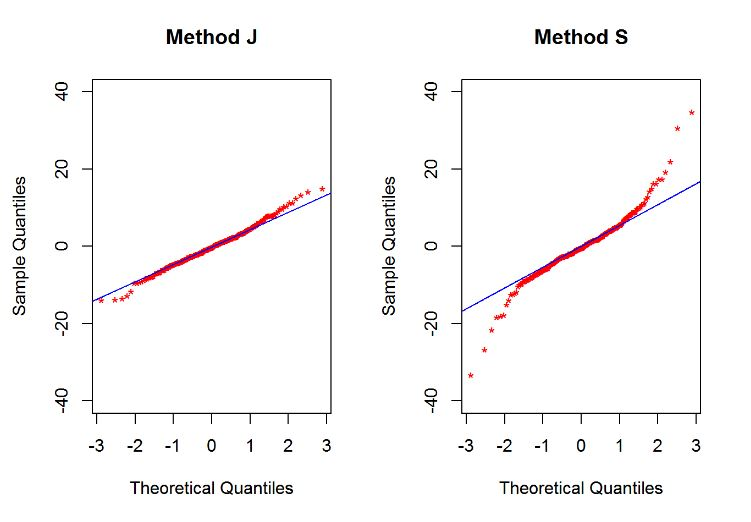
\includegraphics[width=0.9\linewidth]{images/Resid-newplot2}
%		
%	\end{figure}

\begin{framed}
	\begin{verbatim}
	plot(roy.NLME, resid(., type = "p") ~ fitted(.) | method, 
	abline = 0, id=.05)
	\end{verbatim}
\end{framed}
%	\begin{figure}
%		\centering
%		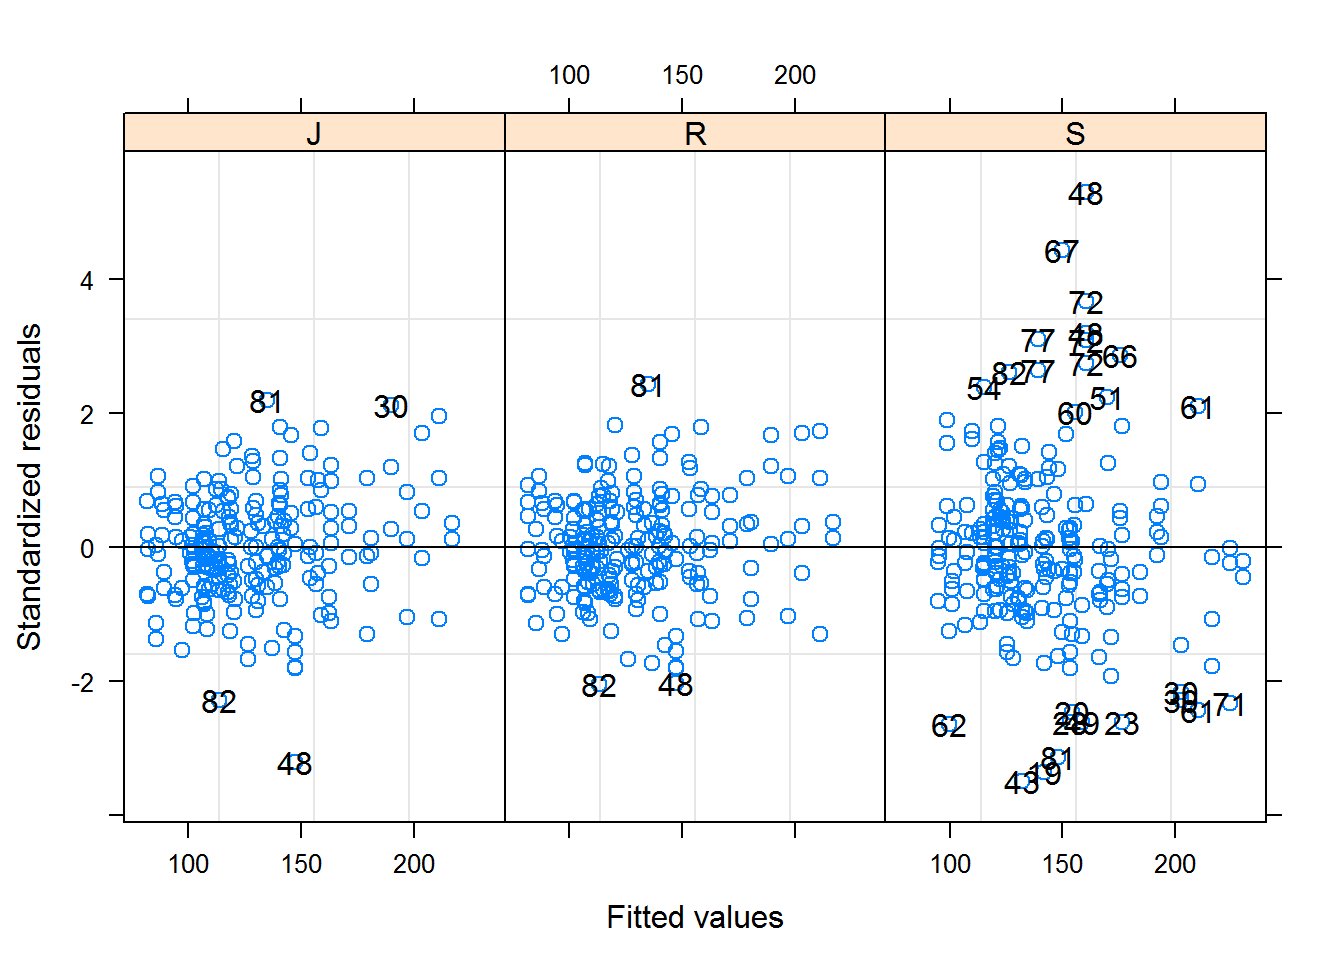
\includegraphics[width=0.9\linewidth]{images/bloodnlmeResidPlot2}
%		\caption{}
%		\label{fig:blood}
%	\end{figure}

\begin{framed}
	\begin{verbatim}
	library(predictMeans)
	CookD(model, group=method, plot=TRUE, idn=5, newwd=FALSE)
	\end{verbatim}
\end{framed}



\begin{framed}
	\begin{verbatim}
	
	blood.red <- blood[!(blood$subject %in% c(68,78,80)),]
	dim(blood.red)
	# 27 observations should be removed.
	
	blood.NLME.red <-lme(BP ~ method-1 , random=~1|subject,data = blood.red)
	plot(blood.NLME.red, resid(., type = "p") ~ fitted(.) | method, abline = 0, id=.05)
	\end{verbatim}
\end{framed}


\begin{framed}
	\begin{verbatim}
	> shapiro.test(resid(JS.roy1)[1:255])
	
	Shapiro-Wilk normality test
	
	data:  resid(JS.roy1)[1:255]
	W = 0.9931, p-value = 0.2852
	\end{verbatim}
\end{framed}

\begin{framed}
	\begin{verbatim}
	> shapiro.test(resid(JS.roy1)[256:510])
	
	Shapiro-Wilk normality test
	
	data:  resid(JS.roy1)[256:510]
	W = 0.9395, p-value = 9.503e-09
	\end{verbatim}
\end{framed}
%	\begin{figure}[h!]
%		\centering
%		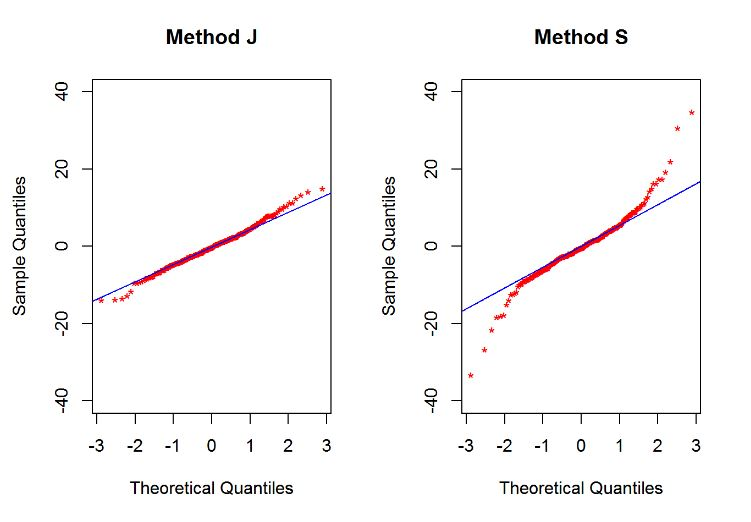
\includegraphics[width=0.9\linewidth]{images/Resid-newplot2}
%		
%	\end{figure}



\begin{framed}
	\begin{verbatim}
	data.frame( response = resid(JS.ARoy20091, type = "response"), 
	pearson  = resid(JS.ARoy20091, type = "pearson"), 
	normalized = resid(JS.ARoy20091, type = "normalized") )
	\end{verbatim}
\end{framed}

\begin{verbatim}
response      pearson    normalized
1    -4.65805902 -0.761587227 -0.7615872269
2    -0.88701342 -0.145025661  0.0776238081
3    -5.16580898 -0.844603753 -0.8446037530
4     2.29041830  0.374480726  0.6450898404
5     7.87508366  1.287567009  1.2875670086
6    -6.57048659 -1.074266908 -1.5090772378
...........................................
\end{verbatim}
For the $J$ observations, the variance is 6.116252 whereas for the $S$ observations, the denominator is 9.118144. (with the expected ratio of  1.490806)


\begin{framed}
	\begin{verbatim}
	> pearson %>%
	+   as.numeric %>% 
	+   matrix(nrow=85) %>%
	+   round(4) 
	[,1]    [,2]    [,3]    [,4]    [,5]    [,6]
	[1,] -0.7616  0.2194  0.3829 -0.2983  0.3597 -0.0790
	[2,] -0.1450  0.1820 -0.1450 -0.5014  0.1567  0.2663
	[3,] -0.8446  0.4634  0.1364 -0.1630 -0.2727  0.1660
	[4,]  0.3745 -0.2795 -0.2795 -0.2658 -0.2658  0.6115
	[5,]  1.2876 -0.6744 -0.6744  0.8935 -0.0935 -0.8612
	[6,] -1.0743  1.8687 -0.7473 -0.0383  0.2908 -0.3673
	...........................................
	
	\end{verbatim}
\end{framed}

We can plot the residuals against the fitted values, to assess the assumption of constant variance. 
\begin{framed}
	\begin{verbatim}
	# standardized residuals versus fitted values 
	plot(JS.ARoy20091, resid(., type = "pearson") ~ fitted(.) , 
	abline = 0, id = 0.05)
	\end{verbatim}
\end{framed}


\begin{framed}
	\begin{verbatim}
	par(mfrow=c(1,2))
	qqnorm((resid(JS.ARoy20091)[1:255]),
	pch="*",col="red",
	ylim=c(-40,40),
	main="Method J")
	qqline(resid(JS.ARoy20091)[1:255],col="blue")
	qqnorm((resid(JS.ARoy20091)[256:510]),
	pch="*",col="red",
	ylim=c(-40,40),
	main="Method S")
	qqline(resid(JS.ARoy20091)[256:510],col="blue")
	par(mfrow=c(1,1))
	\end{verbatim}	
\end{framed}

\subsubsection{Residuals plots}



When the \texttt{plot} function calls the model object, the residual plot is produced.


%====================================================================%


\begin{framed}
	\begin{verbatim}
	plot(JS.roy1, which=c(1) )
	\end{verbatim}
\end{framed}

LME models assume that the residuals of the model are normally distributed. A Normal probability plot can be constructed to check this assumption. Commonly used \texttt{R} commands can be used to construct the plot.


\begin{framed}
	\begin{verbatim}
	qqnorm(resid(JS.roy1),pch="*",col="red")
	qqline(resid(JS.roy1),col="blue")
	\end{verbatim}
\end{framed}

\begin{framed}
	\begin{verbatim}
	table(dat$method[1:255])
	## 
	##   J   S 
	## 255   0
	table(dat$method[256:510])
	## 
	##   J   S 
	##   0 255
	\end{verbatim}	
\end{framed}

\begin{framed}
	\begin{verbatim}
	plot(roy.NLME, resid(., type = "p") ~ fitted(.) | method, 
	abline = 0, id=.05)
	\end{verbatim}
\end{framed}
%	\begin{figure}
%		\centering
%		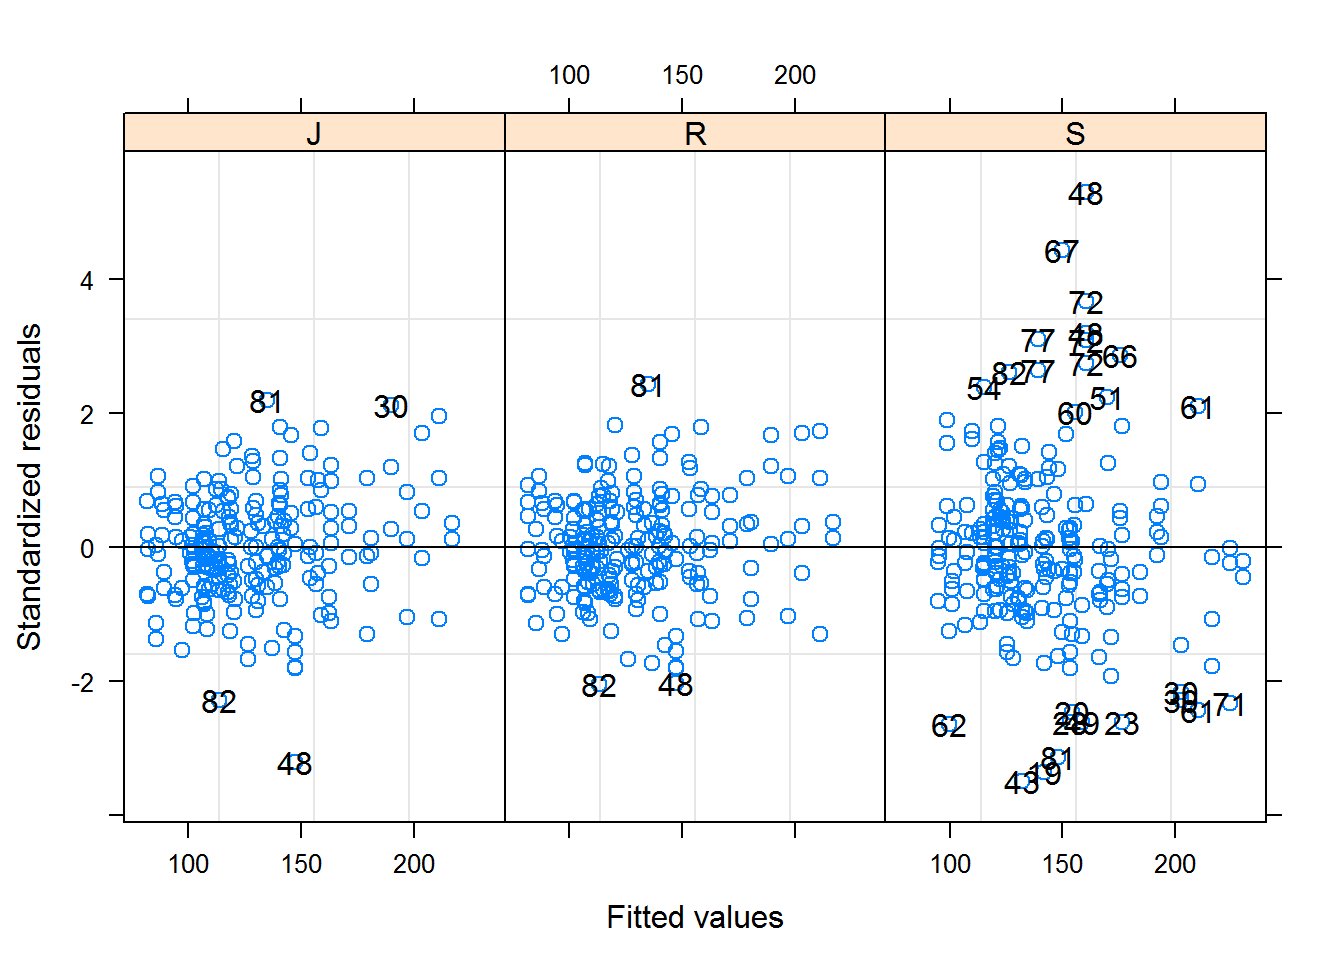
\includegraphics[width=0.9\linewidth]{images/bloodnlmeResidPlot2}
%		\caption{}
%		\label{fig:blood}
%	\end{figure}





\begin{framed}
	\begin{verbatim}
	data.frame( response = resid(JS.ARoy20091, type = "response"), 
	pearson  = resid(JS.ARoy20091, type = "pearson"), 
	normalized = resid(JS.ARoy20091, type = "normalized") )
	\end{verbatim}
\end{framed}

\begin{verbatim}
response      pearson    normalized
1    -4.65805902 -0.761587227 -0.7615872269
2    -0.88701342 -0.145025661  0.0776238081
3    -5.16580898 -0.844603753 -0.8446037530
4     2.29041830  0.374480726  0.6450898404
5     7.87508366  1.287567009  1.2875670086
6    -6.57048659 -1.074266908 -1.5090772378
...........................................
\end{verbatim}
For the $J$ observations, the variance is 6.116252 whereas for the $S$ observations, the denominator is 9.118144. (with the expected ratio of  1.490806)


\begin{framed}
	\begin{verbatim}
	> pearson %>%
	+   as.numeric %>% 
	+   matrix(nrow=85) %>%
	+   round(4) 
	[,1]    [,2]    [,3]    [,4]    [,5]    [,6]
	[1,] -0.7616  0.2194  0.3829 -0.2983  0.3597 -0.0790
	[2,] -0.1450  0.1820 -0.1450 -0.5014  0.1567  0.2663
	[3,] -0.8446  0.4634  0.1364 -0.1630 -0.2727  0.1660
	[4,]  0.3745 -0.2795 -0.2795 -0.2658 -0.2658  0.6115
	[5,]  1.2876 -0.6744 -0.6744  0.8935 -0.0935 -0.8612
	[6,] -1.0743  1.8687 -0.7473 -0.0383  0.2908 -0.3673
	...........................................
	
	\end{verbatim}
\end{framed}

We can plot the residuals against the fitted values, to assess the assumption of constant variance. 
\begin{framed}
	\begin{verbatim}
	# standardized residuals versus fitted values 
	plot(JS.ARoy20091, resid(., type = "pearson") ~ fitted(.) , 
	abline = 0, id = 0.05)
	\end{verbatim}
\end{framed}


\begin{framed}
	\begin{verbatim}
	par(mfrow=c(1,2))
	qqnorm((resid(JS.ARoy20091)[1:255]),
	pch="*",col="red",
	ylim=c(-40,40),
	main="Method J")
	qqline(resid(JS.ARoy20091)[1:255],col="blue")
	qqnorm((resid(JS.ARoy20091)[256:510]),
	pch="*",col="red",
	ylim=c(-40,40),
	main="Method S")
	qqline(resid(JS.ARoy20091)[256:510],col="blue")
	par(mfrow=c(1,1))
	\end{verbatim}	
\end{framed}

This code will allow you to make QQ plots for each level of the random effects.  LME models assume that not only the within-cluster residuals are normally distributed, but that each level of the random effects are as well. Depending on the model, you can vary the level from 0, 1, 2 and so on
\begin{framed}
	\begin{verbatim}
	qqnorm(JS.ARoy20091, ~ranef(.))
	
	# 	qqnorm(JS.ARoy20091, ~ranef(.,levels=1)
	\end{verbatim}
\end{framed}
\begin{figure}[h!]
	\centering
	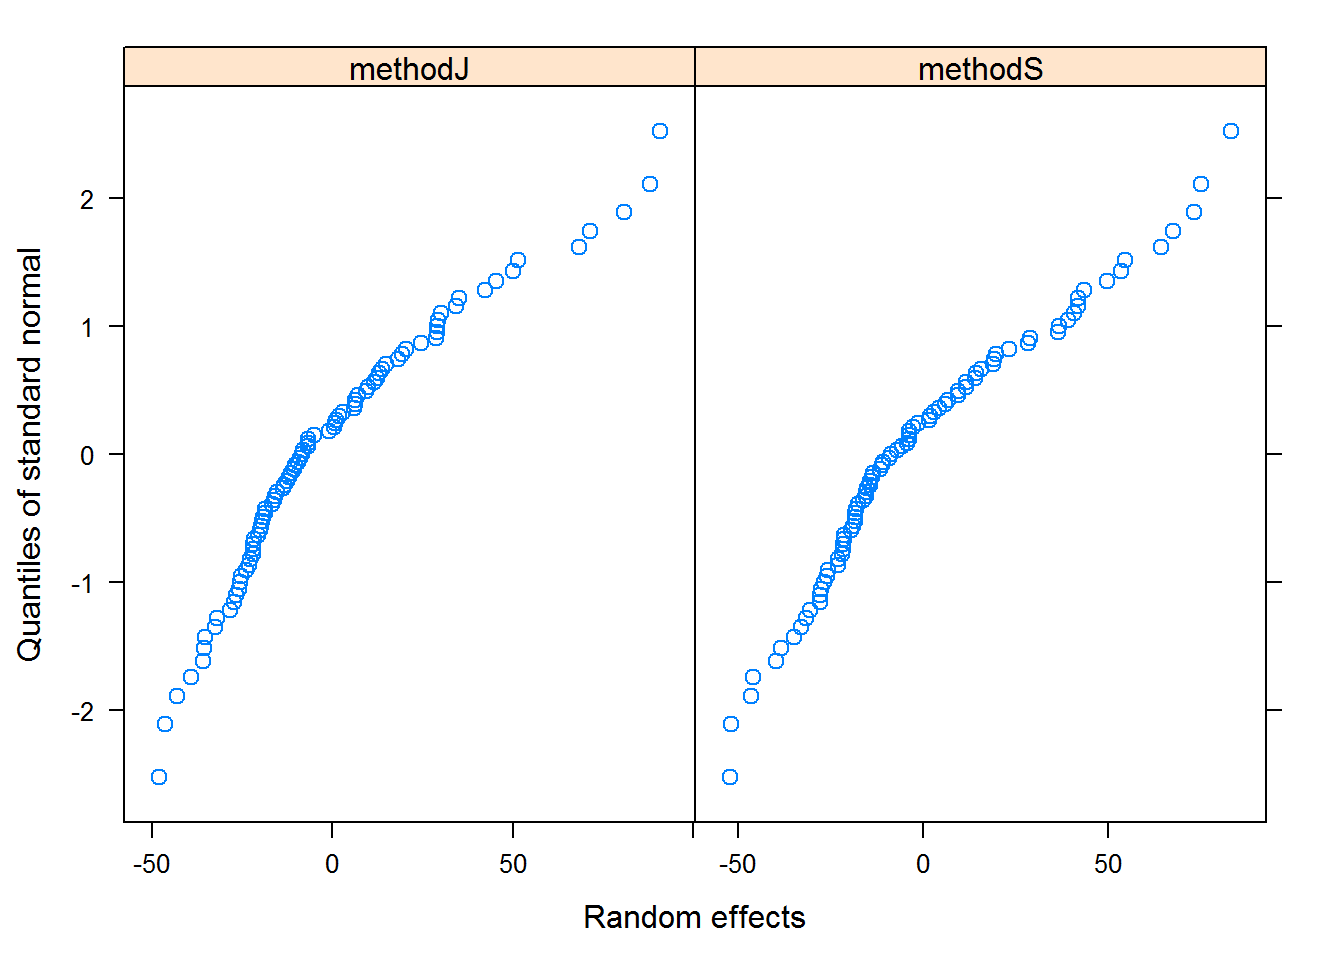
\includegraphics[width=0.9\linewidth]{images/ResidPlot2}
	\caption{}
	\label{fig:ResidPlot2}
\end{figure}	


\begin{framed}
	\begin{verbatim}
	data.frame( response = resid(JS.roy1, type = "response"), 
	pearson  = resid(JS.roy1, type = "pearson"), 
	normalized = resid(JS.roy1, type = "normalized") )
	\end{verbatim}
\end{framed}

\begin{verbatim}
response      pearson    normalized
1    -4.65805902 -0.761587227 -0.7615872269
2    -0.88701342 -0.145025661  0.0776238081
3    -5.16580898 -0.844603753 -0.8446037530
4     2.29041830  0.374480726  0.6450898404
5     7.87508366  1.287567009  1.2875670086
6    -6.57048659 -1.074266908 -1.5090772378
...........................................
\end{verbatim}
For the $J$ observations, the variance is 6.116252 whereas for the $S$ observations, the denominator is 9.118144. (with the expected ratio of  1.490806)


\begin{framed}
	\begin{verbatim}
	> pearson %>%
	+   as.numeric %>% 
	+   matrix(nrow=85) %>%
	+   round(4) 
	[,1]    [,2]    [,3]    [,4]    [,5]    [,6]
	[1,] -0.7616  0.2194  0.3829 -0.2983  0.3597 -0.0790
	[2,] -0.1450  0.1820 -0.1450 -0.5014  0.1567  0.2663
	[3,] -0.8446  0.4634  0.1364 -0.1630 -0.2727  0.1660
	[4,]  0.3745 -0.2795 -0.2795 -0.2658 -0.2658  0.6115
	[5,]  1.2876 -0.6744 -0.6744  0.8935 -0.0935 -0.8612
	[6,] -1.0743  1.8687 -0.7473 -0.0383  0.2908 -0.3673
	...........................................
	
	\end{verbatim}
\end{framed}

We can plot the residuals against the fitted values, to assess the assumption of constant variance. 
\begin{framed}
	\begin{verbatim}
	# standardized residuals versus fitted values 
	plot(JS.roy1, resid(., type = "pearson") ~ fitted(.) , 
	abline = 0, id = 0.05)
	\end{verbatim}
\end{framed}
\begin{figure}[h!]
	\centering
	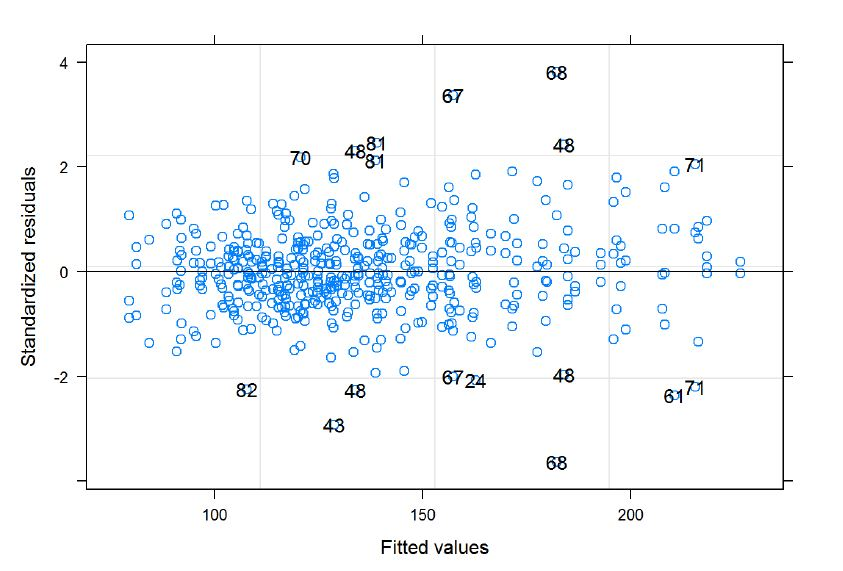
\includegraphics[width=0.9\linewidth]{images/Residuals-JS-Roy}
	\caption{}
	\label{fig:Residuals-JS-Roy}
\end{figure}


\begin{itemize}
	\item
	The \textbf{Scale-Location} plot, also called ‘Spread-Location’ or ‘S-L’ plot, takes the square root of the absolute residuals in order to diminish skewness (sqrt(|E|)) is much less skewed than | E | for Gaussian zero-mean E).
	
	\item
	The \textbf{Residual-Leverage} plot shows contours of equal Cook's distance, for values of cook.levels (by default 0.5 and 1) and omits cases with leverage one with a warning. If the leverages are constant (as is typically the case in a balanced aov situation) the plot uses factor level combinations instead of the leverages for the x-axis. (The factor levels are ordered by mean fitted value.)
\end{itemize}
\begin{framed}
	\begin{verbatim}
	par(mfrow=c(4,1))
	plot(fittedmodel)
	par(opar)
	\end{verbatim}
\end{framed}

%---------------------------------------------------------------------------%
\chapter{Residuals for LME Models}
%-------------------------------------------------------------- %


\section{Diagnostic Tools for the nlme package}


With the nlme package, the generic function \texttt{lme()} fits a linear mixed-effects model in the formulation described in Laird and Ware (1982) but allowing for nested random effects. 

The within-group errors are allowed to be correlated and/or have unequal variances, which is very important in fitting the models for Roy's Tests

The nlme package has a limited set of diagnostic tools that can be used to assess the model fit. A review of the package manual is sufficient to get a sense of the package's capability in that regard.




\section{Computation and Notation } %2.3
with $\boldsymbol{V}$ unknown, a standard practice for estimating $\boldsymbol{X \beta}$ is the estime the variance components $\sigma^2_j$,
compute an estimate for $\boldsymbol{V}$ and then compute the projector matrix $A$, $\boldsymbol{X \hat{\beta}}  = \boldsymbol{AY}$.


%\citet{zewotir} remarks that $\boldsymbol{D}$ is a block diagonal with the $i-$th block being $u \boldsymbol{I}$

\chapter{Model Diagnostics}
%---------------------------------------------------------------------------%
%1.1 Introduction to Influence Analysis
%1.2 Extension of techniques to LME Models
%1.3 Residual Diagnostics
%1.4 Standardized and studentized residuals
%1.5 Covariance Parameters
%1.6 Case Deletion Diagnostics
%1.7 Influence Analysis
%1.8 Terminology for Case Deletion
%1.9 Cook's Distance (Classical Case)
%1.10 Cook's Distance (LME Case)
%1.11 Likelihood Distance
%1.12 Other Measures
%1.13 CPJ Paper
%1.14 Matrix Notation of Case Deletion
%1.15 CPJ's Three Propositions
%1.16 Other measures of Influence
%---------------------------------------------------------------------------%

\section{Extension of techniques to LME Models} %1.2

Model diagnostic techniques, well established for classical models, have since been adapted for use with linear mixed effects models.Diagnostic techniques for LME models are inevitably more difficult to implement, due to the increased complexity.

%% Beckman, Nachtsheim and Cook (1987) \citet{Beckman} applied the local influence method of Cook (1986) to the analysis of the linear mixed model.

While the concept of influence analysis is straightforward, implementation in mixed models is more complex. Update formulae for fixed effects models are available only when the covariance parameters are assumed to be known.

If the global measure suggests that the points in $U$ are influential, the nature of that influence should be determined. In particular, the points in $U$ can affect the following

\begin{itemize}
	\item the estimates of fixed effects,
	\item the estimates of the precision of the fixed effects,
	\item the estimates of the covariance parameters,
	\item the estimates of the precision of the covariance parameters,
	\item fitted and predicted values.
\end{itemize}


%---------------------------------------------------------------------------%
\newpage
\section{Residual diagnostics} %1.3
For classical linear models, residual diagnostics are typically implemented as a plot of the observed residuals and the predicted values. A visual inspection for the presence of trends inform the analyst on the validity of distributional assumptions, and to detect outliers and influential observations.



%--Marginal and Conditional Residuals

\subsection{Residuals diagnostics in mixed models}

%schabenberger
The marginal and conditional means in the linear mixed model are
$E[\boldsymbol{Y}] = \boldsymbol{X}\boldsymbol{\beta}$ and
$E[\boldsymbol{Y|\boldsymbol{u}}] = \boldsymbol{X}\boldsymbol{\beta} + \boldsymbol{Z}\boldsymbol{u}$, respectively.

A residual is the difference between an observed quantity and its estimated or predicted value. In the mixed
model you can distinguish marginal residuals $r_m$ and conditional residuals $r_c$. 


\subsection{Marginal and Conditional Residuals}

A marginal residual is the difference between the observed data and the estimated (marginal) mean, $r_{mi} = y_i - x_0^{\prime} \hat{b}$
A conditional residual is the difference between the observed data and the predicted value of the observation,
$r_{ci} = y_i - x_i^{\prime} \hat{b} - z_i^{\prime} \hat{\gamma}$

In linear mixed effects models, diagnostic techniques may consider `conditional' residuals. A conditional residual is the difference between an observed value $y_{i}$ and the conditional predicted value $\hat{y}_{i} $.

\[ \hat{epsilon}_{i} = y_{i} - \hat{y}_{i} = y_{i} - ( X_{i}\hat{beta} + Z_{i}\hat{b}_{i}) \]

However, using conditional residuals for diagnostics presents difficulties, as they tend to be correlated and their variances may be different for different subgroups, which can lead to erroneous conclusions.

%1.5
%http://support.sas.com/documentation/cdl/en/statug/63033/HTML/default/viewer.htm#statug_mixed_sect024.htm






\begin{equation}
r_{mi}=x^{T}_{i}\hat{\beta}
\end{equation}

	\subsection{Marginal Residuals}
	\begin{eqnarray}
	\hat{\beta} &=& (X^{T}R^{-1}X)^{-1}X^{T}R^{-1}Y \nonumber \\
	&=& BY \nonumber
	\end{eqnarray}

\section{Standardized and studentized residuals} %1.4
%--Studentized and Standardized Residuals

To alleviate the problem caused by inconstant variance, the residuals are scaled (i.e. divided) by their standard deviations. This results in a \index{standardized residual}`standardized residual'. Because true standard deviations are frequently unknown, one can instead divide a residual by the estimated standard deviation to obtain the \index{studentized residual}`studentized residual. 

\subsection{Standardization} %1.4.1

A random variable is said to be standardized if the difference from its mean is scaled by its standard deviation. The residuals above have mean zero but their variance is unknown, it depends on the true values of $\theta$. Standardization is thus not possible in practice.

\subsection{Studentization}
In statistics, a studentized residual is the quotient resulting from the division of a residual by an estimate of its standard deviation. Typically the standard deviations of residuals in a sample vary greatly from one data point to another even when the errors all have the same standard deviation, particularly in regression analysis; thus it does not make sense to compare residuals at different data points without first studentizing. It is a form of a Student's t-statistic, with the estimate of error varying between points.

This is an important technique in the detection of outliers. It is named in honor of William Sealey Gosset, who wrote under the pseudonym Student, and dividing by an estimate of scale is called studentizing, in analogy with standardizing and normalizing: see Studentization.

\subsection{Studentization} %1.4.2
Instead, you can compute studentized residuals by dividing a residual by an estimate of its standard deviation. 

\subsection{Internal and External Studentization} %1.4.3
If that estimate is independent of the $i-$th observation, the process is termed \index{external studentization}`external studentization'. This is usually accomplished by excluding the $i-$th observation when computing the estimate of its standard error. If the observation contributes to the
standard error computation, the residual is said to be \index{internally studentization}internally studentized.

Externally \index{studentized residual} studentized residual require iterative influence analysis or a profiled residuals variance.


\subsection{Computation}%1.4.4

The computation of internally studentized residuals relies on the diagonal entries of $\boldsymbol{V} (\hat{\theta})$ - $\boldsymbol{Q} (\hat{\theta})$, where $\boldsymbol{Q} (\hat{\theta})$ is computed as

\[ \boldsymbol{Q} (\hat{\theta}) = \boldsymbol{X} ( \boldsymbol{X}^{\prime}\boldsymbol{Q} (\hat{\theta})^{-1}\boldsymbol{X})\boldsymbol{X}^{-1} \]

\subsection{Pearson Residual}%1.4.5

Another possible scaled residual is the \index{Pearson residual} `Pearson residual', whereby a residual is divided by the standard deviation of the dependent variable. The Pearson residual can be used when the variability of $\hat{\beta}$ is disregarded in the underlying assumptions.

%---------------------------------------------------------------------------%
\newpage
\section{Covariance Parameters} %1.5
The unknown variance elements are referred to as the covariance parameters and collected in the vector $\theta$.
% - where is this coming from?
% - where is it used again?
% - Has this got anything to do with CovTrace etc?
%---------------------------------------------------------------------------%
\newpage

\section{Effects on fitted and predicted values}
\begin{equation}
\hat{e_{i}}_{(U)} = y_{i} - x\hat{\beta}_{(U)}
\end{equation}

\subsection{Case Deletion Diagnostics for Mixed Models}

\textbf{Christensen} notes the case deletion diagnostics techniques have not been applied to linear mixed effects models and seeks to develop methodologies in that respect.

\textbf{Christensen} develops these techniques in the context of REML

\subsection{Methods and Measures}
The key to making deletion diagnostics useable is the development of efficient computational formulas, allowing one to obtain the \index{case deletion diagnostics} case deletion diagnostics by making use of basic building blocks, computed only once for the full model.

\textbf{Zewotir} lists several established methods of analyzing influence in LME models. These methods include 
\begin{itemize}
	\item Cook's distance for LME models,
	\item \index{likelihood distance} likelihood distance,
	\item the variance (information) ration,
	\item the \index{Cook-Weisberg statistic} Cook-Weisberg statistic,
	\item the \index{Andrews-Prebigon statistic} Andrews-Prebigon statistic.
\end{itemize}


%---------------------------------------------------------------------------%
\newpage
\section{Influence analysis} %1.7

Likelihood based estimation methods, such as ML and REML, are sensitive to unusual observations. Influence diagnostics are formal techniques that assess the influence of observations on parameter estimates for $\beta$ and $\theta$. A common technique is to refit the model with an observation or group of observations omitted.

\textbf{west} examines a group of methods that examine various aspects of influence diagnostics for LME models. For overall influence, the most common approaches are the `likelihood distance' and the `restricted likelihood distance'.

\subsection{Cook's 1986 paper on Local Influence}%1.7.1
Cook 1986 introduced methods for local influence assessment. These methods provide a powerful tool for examining perturbations in the assumption of a model, particularly the effects of local perturbations of parameters of observations.

The local-influence approach to influence assessment is quitedifferent from the case deletion approach, comparisons are of interest.



\subsection{Overall Influence}
An overall influence statistic measures the change in the objective function being minimized. For example, in
OLS regression, the residual sums of squares serves that purpose. In linear mixed models fit by
\index{maximum likelihood} maximum likelihood (ML) or \index{restricted maximum likelihood} restricted maximum likelihood (REML), an overall influence measure is the \index{likelihood distance} likelihood distance [Cook and Weisberg ].

%--------------------------------------------------------------------------%
\newpage

\section{Likelihood Distance} %1.11
The likelihood distance gives the amount by which the log-likelihood of the full data changes if one were
to evaluate it at the reduced-data estimates. The important point is that $l(\psi_{(U)})$ is not the log-likelihood
obtained by fitting the model to the reduced data set.

It is obtained by evaluating the likelihood function based on the full data set (containing all n observations) at the reduced-data estimates.

The likelihood distance is a global, summary measure, expressing the joint influence of the observations in
the set $U$ on all parameters in $\psi$  that were subject to updating.
%------------%

\subsection{Likelihood Distance}

The \index{likelihood distance} likelihood distance is a global, summary measure, expressing the joint influence of the observations in the set $U$ on all parameters in $\phi$  that were subject to updating.




%---------------------------------------------------------------------------%

\section{Iterative and non-iterative influence analysis} %1.13
\textbf{schabenberger} highlights some of the issue regarding implementing mixed model diagnostics.

A measure of total influence requires updates of all model parameters.

however, this doesnt increase the procedures execution time by the same degree.
\subsection{Iterative Influence Analysis}

%----schabenberger page 8
For linear models, the implementation of influence analysis is straightforward.
However, for LME models, the process is more complex. Update formulas for the fixed effects are available only when the covariance parameters are assumed to be known. A measure of total influence requires updates of all model parameters.
This can only be achieved in general is by omitting observations, then refitting the model.

\textbf{schabenberger} describes the choice between \index{iterative influence analysis} iterative influence analysis and \index{non-iterative influence analysis} non-iterative influence analysis.


%----------------------------------------------------------------------------------------%



\section{Measures of Influence} %1.16

The impact of an observation on a regression fitting can be determined by the difference between the estimated regression coefficient of a model with all observations and the estimated coefficient when the particular observation is deleted. The measure DFBETA is the studentized value of this difference.

Influence arises at two stages of the LME model. Firstly when $V$ is estimated by $\hat{V}$, and subsequent
estimations of the fixed and random regression coefficients $\beta$ and $u$, given $\hat{V}$.


\subsection{DFFITS} %1.16.1
DFFITS is a statistical measured designed to a show how influential an observation is in a statistical model. It is closely related to the studentized residual.
\begin{displaymath} DFFITS = {\widehat{y_i} -
	\widehat{y_{i(k)}} \over s_{(k)} \sqrt{h_{ii}}} \end{displaymath}


\subsection{PRESS} %1.16.2
The prediction residual sum of squares (PRESS) is an value associated with this calculation. When fitting linear models, PRESS can be used as a criterion for model selection, with smaller values indicating better model fits.
\begin{equation}
PRESS = \sum(y-y^{(k)})^2
\end{equation}


\begin{itemize}
	\item $e_{-Q} = y_{Q} - x_{Q}\hat{\beta}^{-Q}$
	\item $PRESS_{(U)} = y_{i} - x\hat{\beta}_{(U)}$
\end{itemize}

\subsection{DFBETA} %1.16.3
\begin{eqnarray}
DFBETA_{a} &=& \hat{\beta} - \hat{\beta}_{(a)} \\
&=& B(Y-Y_{\bar{a}}
\end{eqnarray}
%-------------------------------------------------------------------------------------------------------------------------------------%
%-------------------------------------------------------------------------------------------------------------------------------------%
%-------------------------------------------------------------------------------------------------Chapter 2	------------------------%
	
	%--Marginal and Conditional Residuals
	
	%========================================================================================== %
	\subsection{Residuals diagnostics in LME Models}
	
	
	A residual is the difference between an observed quantity and its
	estimated or predicted value. In LME models, there are two types
	of residuals, marginal residuals and conditional residuals. 
	In a model without random effects, both sets of residuals coincide. schabenberger provides a useful summary. 
	% \subsection{Marginal and Conditional Residuals}
	
	\begin{itemize}
		\item A marginal residual is the difference between the observed data and the estimated (marginal) mean, $r_{mi} = y_i - x_0^{\prime} \hat{b}$
		\item A conditional residual is the difference between an observed value $y_{i}$ and the conditional predicted value $\hat{y}_{i} $,
		\[r_{ci} = y_i - x_i^{\prime} \hat{b} - z_i^{\prime} \hat{\gamma}\]
	\end{itemize} 
	
	%schabenberger
	The marginal and conditional means in the linear mixed model are
	$E[\boldsymbol{Y}] = \boldsymbol{X}\boldsymbol{\beta}$ and
	$E[\boldsymbol{Y|\boldsymbol{u}}] = \boldsymbol{X}\boldsymbol{\beta} + \boldsymbol{Z}\boldsymbol{u}$, respectively.
	%1.5
	%http://support.sas.com/documentation/cdl/en/statug/63033/HTML/default/viewer.htm#statug_mixed_sect024.htm
	
	\subsection{Marginal and Conditional Residuals}
	
	A marginal residual is the difference between the observed data and the estimated (marginal) mean, $r_{mi} = y_i - x_0^{\prime} \hat{b}$
	A conditional residual is the difference between the observed data and the predicted value of the observation,
	$r_{ci} = y_i - x_i^{\prime} \hat{b} - z_i^{\prime} \hat{\gamma}$
	
	In linear mixed effects models, diagnostic techniques may consider `conditional' residuals. A conditional residual is the difference between an observed value $y_{i}$ and the conditional predicted value $\hat{y}_{i} $.
	
	\[ \hat{epsilon}_{i} = y_{i} - \hat{y}_{i} = y_{i} - ( X_{i}\hat{beta} + Z_{i}\hat{b}_{i}) \]
	
	However, using conditional residuals for diagnostics presents difficulties, as they tend to be correlated and their variances may be different for different subgroups, which can lead to erroneous conclusions.
	
	
	
	
	
	
	
	\begin{equation}
	r_{mi}=x^{T}_{i}\hat{\beta}
	\end{equation}
	

	\subsection{Marginal and Conditional Residuals}
	
	
	A marginal residual is the difference between the observed data and the estimated (marginal) mean, $r_{mi} = y_i - x_0^{\prime} \hat{b}$
	A conditional residual is the difference between the observed data and the predicted value of the observation,
	$r_{ci} = y_i - x_i^{\prime} \hat{b} - z_i^{\prime} \hat{\gamma}$
	
	
	In linear mixed effects models, diagnostic techniques may consider `conditional' residuals. A conditional residual is the difference between an observed value $y_{i}$ and the conditional predicted value $\hat{y}_{i} $.
	
	
	\[ \hat{epsilon}_{i} = y_{i} - \hat{y}_{i} = y_{i} - ( X_{i}\hat{beta} + Z_{i}\hat{b}_{i}) \]
	
	
	However, using conditional residuals for diagnostics presents difficulties, as they tend to be correlated and their variances may be different for different subgroups, which can lead to erroneous conclusions.
	
	
	%1.5
	%http://support.sas.com/documentation/cdl/en/statug/63033/HTML/default/viewer.htm#statug_mixed_sect024.htm
	
	
	
	\subsection{Residuals diagnostics in LME Models}
	
	%schabenberger
	The marginal and conditional means in the linear mixed model are
	$E[\boldsymbol{Y}] = \boldsymbol{X}\boldsymbol{\beta}$ and
	$E[\boldsymbol{Y|\boldsymbol{u}}] = \boldsymbol{X}\boldsymbol{\beta} + \boldsymbol{Z}\boldsymbol{u}$, respectively.
	
	
	
	
	
	
	
	
	
	
	\begin{equation}
	r_{mi}=x^{T}_{i}\hat{\beta}
	\end{equation}
	
	
	\subsection{Marginal Residuals}
	\begin{eqnarray}
	\hat{\beta} &=& (X^{T}R^{-1}X)^{-1}X^{T}R^{-1}Y \nonumber \\
	&=& BY \nonumber
	\end{eqnarray}
	
	
	
	
	
	%------------------------------------------------------------%
	\section*{Residuals}
	
	Residuals are used to examine model assumptions and to detect outliers and potentially influential data
	point. The raw residuals $r_{mi}$ and $r_{ci}$ are usually not well suited for these purposes.
	
	\begin{itemize}
		\item Conditional Residuals $r_{ci}$
		\item Marginal Residuals $r_{mi}$
		\item 
	\end{itemize}
	
	\subsection*{Marginal Residuals}
	
	%------------------------------------------------------------%

	Distinction From Linear Models
	\begin{itemize}
		\item The differences between perturbation and residual analysis in the linear model and the linear mixed model
		are connected to the important facts that b and b
		depend on the estimates of the covariance parameters,
		that b has the form of an (estimated) generalized least squares (GLS) estimator, and that 
		is a random
		vector.
		\item In a mixed model, you can consider the data in a conditional and an unconditional sense. If you imagine
		a particular realization of the random effects, then you are considering the conditional distribution
		Y|
		\item If you are interested in quantities averaged over all possible values of the random effects, then
		you are interested in Y; this is called the marginal formulation. In a clinical trial, for example, you
		may be interested in drug efficacy for a particular patient. If random effects vary by patient, that is a
		conditional problem. If you are interested in the drug efficacy in the population of all patients, you are
		using a marginal formulation. Correspondingly, there will be conditional and marginal residuals, for
		example.
		\item The estimates of the fixed effects  depend on the estimates of the covariance parameters. If you are
		interested in determining the influence of an observation on the analysis, you must determine whether
		this is influence on the fixed effects for a given value of the covariance parameters, influence on the
		covariance parameters, or influence on both.
		\item Mixed models are often used to analyze repeated measures and longitudinal data. The natural experimental
		or sampling unit in those studies is the entity that is repeatedly observed, rather than each
		individual repeated observation. For example, you may be analyzing monthly purchase records by
		customer. 
		\item An influential “data point” is then not necessarily a single purchase. You are probably more
		interested in determining the influential customer. This requires that you can measure the influence
		of sets of observations on the analysis, not just influence of individual observations.
		\item The computation of case deletion diagnostics in the classical model is made simple by the fact that
		%estimates of  and 2, which exclude the ith observation, can be %computed without re-fitting the
		model. Such update formulas are available in the mixed model only if you assume that the covariance
		parameters are not affected by the removal of the observation in question. This is rarely a reasonable
		assumption.
		\item The application of well-known concepts in model-data diagnostics to the mixed model can produce results
		that are at first counter-intuitive, since our understanding is steeped in the ordinary least squares
		(OLS) framework. As a consequence, we need to revisit these important concepts, ask whether they
		are “portable” to the mixed model, and gain new appreciation for their changed properties. An important
		example is the ostensibly simple concept of leverage. 
		\item The definition of leverage adopted by
		the MIXED procedure can, in some instances, produce negative values, which are mathematically
		impossible in OLS. Other measures that have been proposed may be non-negative, but trade other
		advantages. Another example are properties of residuals. While OLS residuals necessarily sum to
		zero in any model (with intercept), this not true of the residuals in many mixed models.
	\end{itemize}
	\newpage
	%---------------------------------------------------------------------------%
	\newpage
	\section{Residual diagnostics} %1.3
	For classical linear models, residual diagnostics are typically implemented as a plot of the observed residuals and the predicted values. A visual inspection for the presence of trends inform the analyst on the validity of distributional assumptions, and to detect outliers and influential observations.
	
	
	
	%--Marginal and Conditional Residuals
	
	\subsection{Residuals diagnostics in mixed models}
	
	%schabenberger
	The marginal and conditional means in the linear mixed model are
	$E[\boldsymbol{Y}] = \boldsymbol{X}\boldsymbol{\beta}$ and
	$E[\boldsymbol{Y|\boldsymbol{u}}] = \boldsymbol{X}\boldsymbol{\beta} + \boldsymbol{Z}\boldsymbol{u}$, respectively.
	
	A residual is the difference between an observed quantity and its estimated or predicted value. In the mixed
	model you can distinguish marginal residuals $r_m$ and conditional residuals $r_c$. 
	
	
	
	
	
	
	
	
	\begin{equation}
	r_{mi}=x^{T}_{i}\hat{\beta}
	\end{equation}

%======================================================================%
	
	\subsection{Marginal Residuals}
	\begin{eqnarray}
	\hat{\beta} &=& (X^{T}R^{-1}X)^{-1}X^{T}R^{-1}Y \nonumber \\
	&=& BY \nonumber
	\end{eqnarray}
	
	
	\section{Conditional and Marginal Residuals}
	Conditional residuals include contributions from both fixed and random effects, whereas marginal residuals include contribution from only fixed effects.
	
	Suppose the linear mixed-effects model lme has an $n \times p$ fixed-effects design matrix $\boldsymbol{X}$ and an $n \times q$ random-effects design matrix $\boldsymbol{Z}$. 
	
	Also, suppose the p-by-1 estimated fixed-effects vector is $\hat{\beta}$ , and the q-by-1 estimated best linear unbiased predictor (BLUP) 
	vector of random effects is $\hat{b}$ . The fitted conditional response is
	
	\[ \hat{y}_{Cond} = X \hat{\beta} + Z \hat{b} \]
	
	and the fitted marginal response is
	
	
	\[ \hat{y}_{Mar} = X \hat{\beta} \]
	
	residuals can return three types of residuals:
	\begin{itemize} 
		\item raw, 
		\item Pearson, and 
		\item standardized.\end{itemize} For any type, you can compute the conditional or the marginal residuals. For example, the conditional raw residual is
	
	
	\[ r_{Cond} = y - X \hat{\beta} - Z \hat{b} \]
	
	and the marginal raw residual is
	
	
	
	\[ r_{Mar} = y - X \hat{\beta} \]
	
	\newpage
	%=================================================== %
	% http://www.ime.usp.br/~jmsinger/MAE0610/Mixedmodelresiduals.pdf
	
	Cox and Snell (1968, JRSS-B): general definition of residuals for
	models with single source of variability
	Hilden-Minton (1995, PhD thesis UCLA), Verbeke and Lesaffre
	(1997, CSDA) or Pinheiro and Bates (2000, Springer): extension to
	define three types of residuals that accommodate the extra source of
	variability present in linear mixed models, namely:
	
	i) Marginal residuals, 
	%bξ = y − X\hat{\beta} = \hat{M}^{-1}\hat{Q}y ,
	
	predictors of marginal errors, 
	
	%ξ = y − E[y] = y − X\beta = Zb + e
	
	ii) Conditional residuals, 
	\[be = y − X\hat{\beta} − Zbb = \hat{\sigma}Q\hat{y}\] , predictors of
	conditional errors 
	\[e = y − E[y|b] = y − X\beta − Zb\]
	
	iii) BLUP, Zbb, predictors of random effects,
	\[ Zb = E[y|b] − E[y]\]
	
	
	%------------------------------------------------------------------%
	\newpage
	
	\subsection*{Marginal residuals}
	
	\[y - X\beta = Z \eta +\epsilon \]
	\begin{itemize}
		\item
		Should be mean 0, but may show grouping structure
		\item
		May not be homoskedastic.
		\item
		Good for checking fixed effects, just like linear regr.
	\end{itemize}
	%----------------------------------------------------%
	\subsection*{Conditional residuals}
	\[y - X\beta - Z \eta = \epsilon \]
	\begin{itemize}
		\item
		Should be mean zero with no grouping structure
		\item
		Should be homoscedastic.
		\item
		Good for checking normality of outliers
	\end{itemize}
	
	%-----------------------------------------------------%
	\subsection*{Random effects}
	\[y - X\beta -\epsilon = Z \eta \]
	\begin{itemize}
		\item
		Should be mean zero with no grouping structure
		\item
		May not be be homoscedastic.
	\end{itemize}
	
	\section{Residual diagnostics} %1.3
	For classical linear models, residual diagnostics are typically implemented as a plot of the observed residuals and the predicted values. A visual inspection for the presence of trends inform the analyst on the validity of distributional assumptions, and to detect outliers and influential observations.
	
	
	
	%--Marginal and Conditional Residuals
	

	\subsection{Marginal Residuals}
	\begin{eqnarray}
	\hat{\beta} &=& (X^{T}R^{-1}X)^{-1}X^{T}R^{-1}Y \nonumber \\
	&=& BY \nonumber
	\end{eqnarray}
	
	
	
	
	\subsection{Confounded Residuals}
	Hilden-Minton (1995, PhD thesis, UCLA): residual is pure for a
	specific type of error if it depends only on the fixed components and
	on the error that it is supposed to predict
	Residuals that depend on other types of errors are called \textit{\textbf{confounded
			residuals}}
	






\bibliographystyle{chicago}
\bibliography{DB-txfrbib}

\end{document} 